\documentclass[11pt]{article}
\usepackage[italian]{babel}
\usepackage{amsmath, amsfonts}
\usepackage{graphicx}
\begin{document}
\title{\Large Componenti fortemente connesse e visita in profondità}\date{}
\author{Athos Innocenti}
\maketitle
\section{Introduzione}
In questa relazione vengono presentati la visita in profondità di un grafo e l'algoritmo che consente di determinare le componenti fortemente connesse di un grafo orientato.

Nell'analisi delle componenti fortemente connesse si valuta la relazione che sussiste tra l'aumento della probabilità di avere un arco tra due nodi del grafo e il numero di componenti fortemente connesse trovate.

Per la visita in profondità, invece, si valuta la relazione tra l'aumento della probabilità di avere un arco e il numero di radici nel primo attraversamento.
\section{Visita in profondità - DFS}
La \textbf{visita in profondità} su di un grafo orientato ispeziona il grafo scoprendo, uno alla volta, tutti i nodi raggiungibili da un nodo di partenza detto \textit{nodo sorgente}. A ciascun nodo \textit{v} del grafo vengono associati due attributi temporali detti \textit{tempo di scoperta}, indicato con \textit{v.d}, e \textit{tempo di completamento}, indicato con \textit{v.f}. Completata la visita, si avrà in output un insieme di alberi detto \textit{foresta DF} definita in funzione dell'ordine in cui i nodi del grafo sono stati scoperti. Il tempo di esecuzione della procedura DFS è $\Theta(V + E)$ poiché visita ogni nodo e ogni arco del grafo.
\subsection{Analisi DFS}
Per poter analizzare la procedura si considerano tre dimensioni del grafo: un grafo con $25$ nodi, uno con $100$ e un terzo grafo avente $500$ nodi. La probabilità cresce da $0$ a $100$ per il grafo con $25$ nodi, da $0$ a $50$ per il grafo con $100$ nodi e da $0$ a $25$ per il grafo con $500$ nodi. Inoltre, per ciascun valore della probabilità vengono eseguite $10$ prove sulle quali viene fatta una media.
\begin{figure}[p]
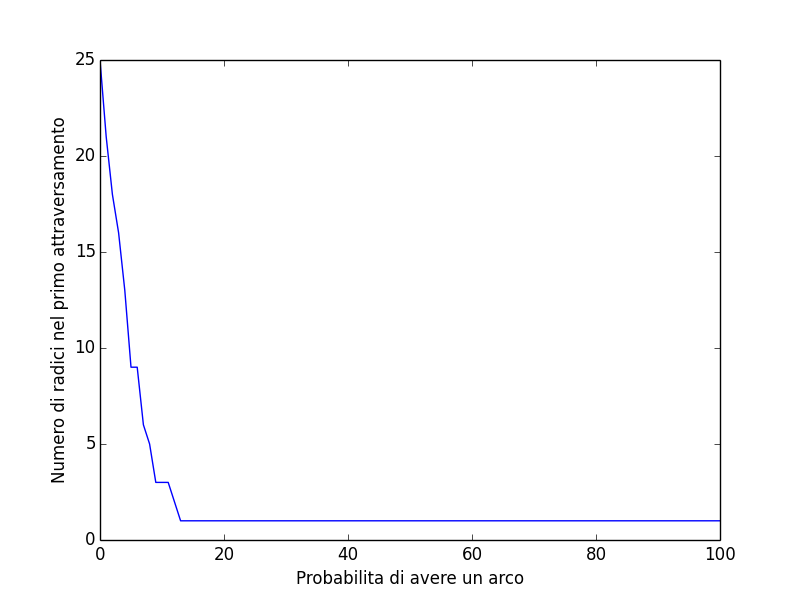
\includegraphics[scale=0.33,angle=0]{radici25.png}
\centering
\caption{Radici nella visita in profondità in un grafo di dimensione 25}
\label{radici25}
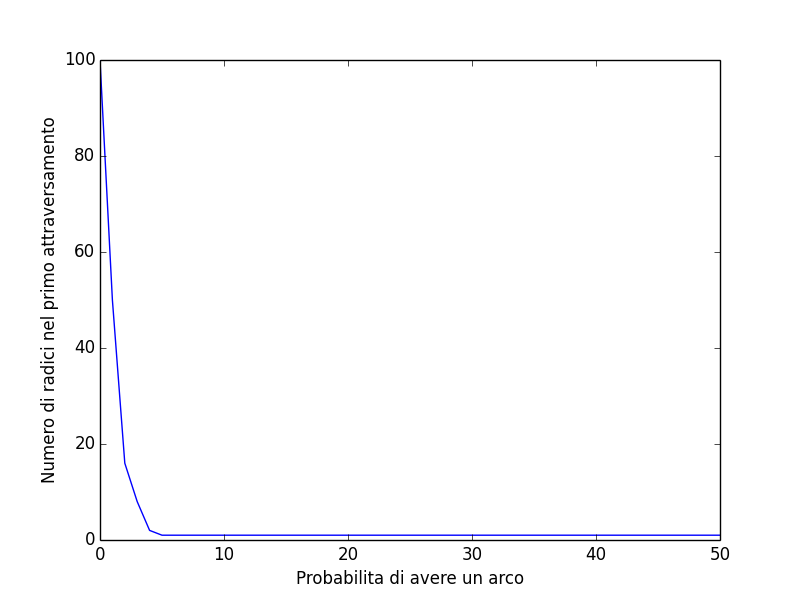
\includegraphics[scale=0.33,angle=0]{radici100.png}
\centering
\caption{Radici nella visita in profondità in un grafo di dimensione 100}
\label{radici100}
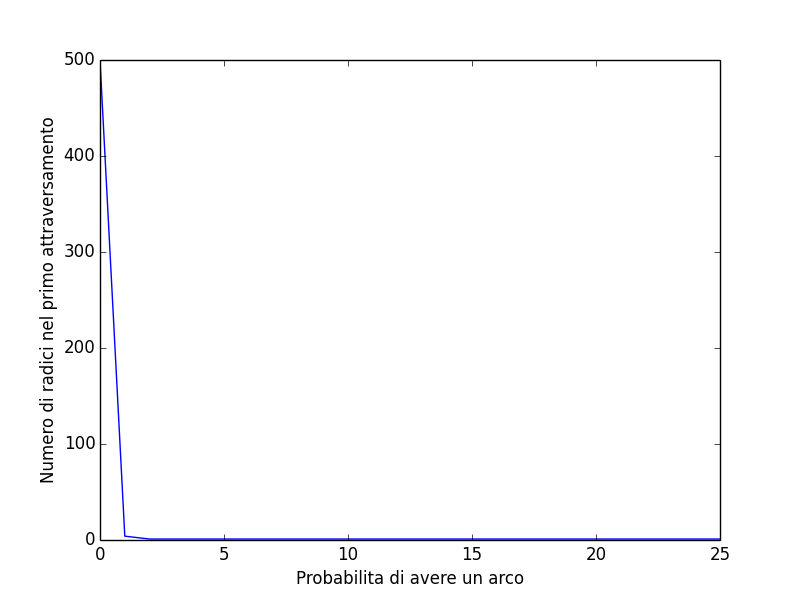
\includegraphics[scale=0.33,angle=0]{radici500.png}
\centering
\caption{Radici nella visita in profondità in un grafo di dimensione 500}
\label{radici500}
\end{figure}
\newline
In riferimento ai grafici in figura \ref{radici25}, \ref{radici100} e \ref{radici500} si nota che all'aumentare della probabilità di avere archi diminuisce il numero di radici nel primo attraversamento DFS, ovvero diminuiscono il numero di alberi nella foresta DF. Il numero di radici tende velocemente ad $1$ e con l'aumentare del numero dei nodi nel grafo, tende a $1$ per valori sempre più piccoli di probabilità.
\section{Componenti fortemente connesse}
Una \textbf{componente fortemente connessa} o \textbf{SCC} di un grafo orientato, è un insieme massimale di vertici tale che, per ogni coppia di vertici \textit{u} e \textit{v} appartenenti all'insieme, esistono due cammini $u \rightsquigarrow v$ e $v \rightsquigarrow u$; ovvero \textit{u} e \textit{v} sono raggiungibili l'uno dall'altro.

L'algoritmo che consente di determinare le componenti fortemente connesse di un grafo orientato \textit{G} esegue i seguenti passi:
\begin{enumerate}
\item Esegue una prima visita in profondità su tale grafo per poter calcolare i tempi di completamento \textit{v.f} per ciascun vertice del grafo
\item Calcola il grafo trasposto $G^T$
\item Esegue una nuova visita in profondità su $G^T$ esaminando i vertici secondo l'ordine decrescente dei tempi di completamento. Le SCC sono quindi gli alberi nella foresta DF ottenuti nella seconda DFS
\end{enumerate}
\subsection{Analisi algoritmo SCC}
Anche per l'analisi dell'algoritmo per trovare le SCC si considera un grafo con $25$, $100$ e $500$ nodi. La probabilità cresce secondo il criterio utilizzato nell'analisi della DFS, eseguendo $10$ prove per ciascun valore, sulle quali viene fatta una media.

Come è possibile vedere dai grafici in figura \ref{scc25}, \ref{scc100} e \ref{scc500}, all'aumentare della probabilità di avere archi si ha una diminuzione del numero di componenti fortemente connesse che corrisponde ad una diminuzione del numero di alberi nella foresta DF nel secondo DFS. In particolare si nota che con l'aumento della probabilità di avere archi, il numero di componenti fortemente connesse tende velocemente a $1$ e all'aumentare del numero di nodi, si raggiunge un'unica componente fortemente connessa per valori sempre più piccoli di probabilità. Guardando i grafici, per il grafo con $25$ nodi il numero di SCC si stabilizza ad $1$ per probabilità pari circa a $20$, nel grafo con $100$ nodi da una probabilità di $5$ e nel grafo con $500$ nodi già per probabilità uguale a $2$ si ottiene un'unica componente fortemente connessa.
\begin{figure}[p]
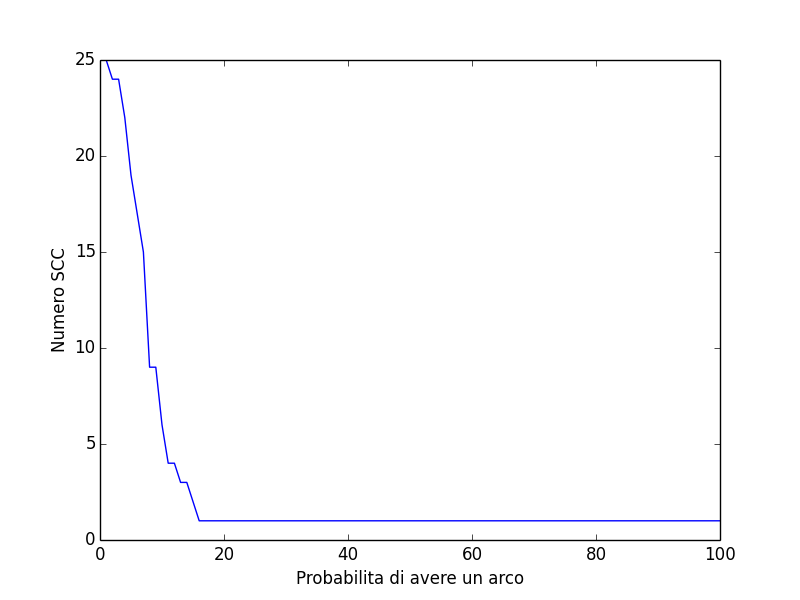
\includegraphics[scale=0.33,angle=0]{scc25.png}
\centering
\caption{Componenti fortemente connesse in un grafo di dimensione 25}
\label{scc25}
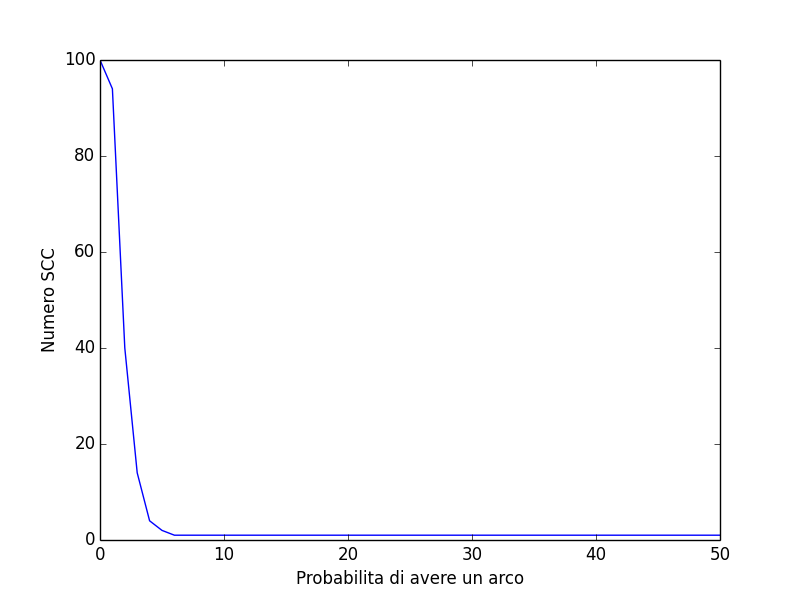
\includegraphics[scale=0.33,angle=0]{scc100.png}
\centering
\caption{Componenti fortemente connesse in un grafo di dimensione 100}
\label{scc100}
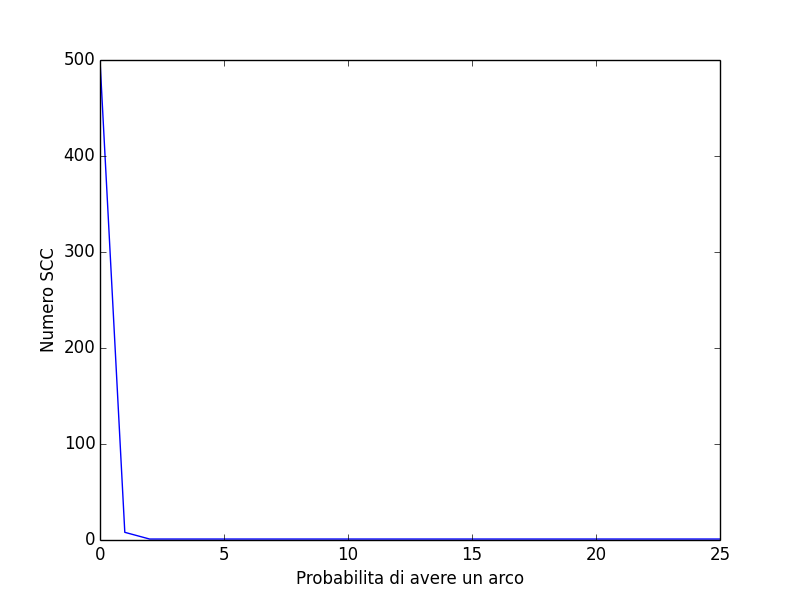
\includegraphics[scale=0.33,angle=0]{scc500.png}
\centering
\caption{Componenti fortemente connesse in un grafo di dimensione 500}
\label{scc500}
\end{figure}
\section{Conclusioni}
Tramite i dati ricavati dalle varie prove è possibile verificare che all'aumentare della probabilità di avere archi, il numero di componenti fortemente connesse diminuisce tendendo a $1$. Questo perché aumentando il numero di archi è più probabile che un nodo sia raggiungibile da un altro e quindi è più probabile che il grafo sia un'unica componente fortemente connessa. Anche la dimensione del grafo, ovvero il suo numero di nodi, influisce sulla velocità con cui il numero di componenti fortemente connesse si stabilizza ad $1$: maggiore è la dimensione del grafo e più velocemente e per valori di probabilità sempre più piccoli si arriva ad avere una sola componente fortemente connessa.

I test sono stati eseguiti su un Macbook Pro con processore 2,7 GHz Intel Core i5, RAM 8 GB 1867 MHz DDR3 e sistema operativo macOS Mojave 10.14.6.
\end{document}